
\section{Wavelet transform}
\label{sec:wavelet_transform}

Due to the frequency-energy dependence of nonlinear vibrations, giving time
varying frequencies for sine sweeps, the Fourier transform(FT), eq.
\eqref{eq:ft_transform} does not give useful results.
To allow for a varying frequency the Short Time Fourier transform(STFT) can be
used, eq. \eqref{eq:sft_transform}. Here the function to be transformed is
multiplied by a window function $w(t-\tau)$ which is nonzero only for a short
period of time. Practically this correspond to dividing the original signal into
shorter segments of equal length and then calculate the FT of each segments,
giving a 2D representation of the time-varying spectrum.

Often one want a window observation window that changes with frequency. A short
window gives good time resolution, allowing for identification of when frequency
content changes but poor frequency resolution. On the other hand a long window
allows the frequencies to be identified but gives poor time resolution. One such
window that gives a varying length is the Gaussian window function. Used with
STFT, the transfer is called a Morlet wavelet(MW), eq. \eqref{eq:mw_transform}


\begin{align}
  X(\omega) &= \int_{-\infty}^\infty x(t) e^{-i\omega t} \d t
              \label{eq:ft_transform}\\
  X(\omega, \tau) &= \int_{-\infty}^\infty x(t) w(t-\tau)  e^{-i\omega t} \d t
                    \label{eq:sft_transform}\\
  X(a, b) &= \frac{1}{\sqrt{a}} \int_{-\infty}^\infty x(t) \psi\left(\frac{t-b}{a} \right) \d t
            \label{eq:mw_transform}
\end{align}

For the Morlet wavelet the window function is a Gaussian windowed complex
sinusoidal, $\psi(t) = e^{-t^2/2}e^{i\omega t}$. $a$ defines the frequency
resolution by expanding/contracting the window, see figure
\ref{fig:mw_window_length} and, $b$ is the location of the observation window in
the time domain.

\begin{figure}[!ht]
  \centering
  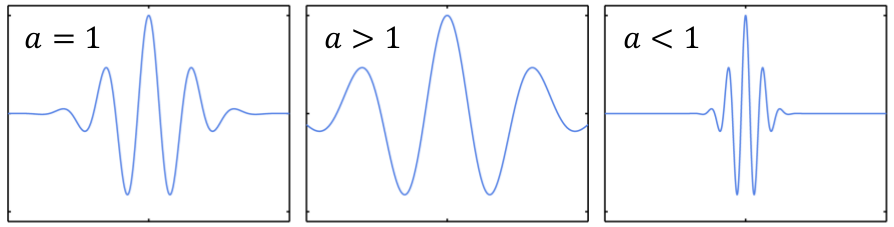
\includegraphics[width=0.8\textwidth]{wt/window_length.png}
  \caption{Influence of $a$ on the window length. Copied from slides given at
    ULG in Liege, Belgium}
  \label{fig:mw_window_length}
\end{figure}


\subsection{Example}
\label{sec:wt_example}

% Figure .. shows a simple example of FT compared to MW for free decay vibrations given by

% \begin{equation}
%   \label{eq:mw_eom}
%   \ddot x + 0.05 \dot x + 0.5 x + x^3 = 0, \quad x_0 = 10, \quad \dot x_0 = 0
% \end{equation}
Figure \ref{fig:mw_2dof}(a) shows the wavelet transform of the coupled duffing
system. Fig \ref{fig:mw_2dof}(b) shows the linear transform for comparison and
fig \ref{fig:mw_2dof}(c) the sweep. For the linear system, the two fundamental
frequencies $\omega_1$ and $\omega_2$ along with the excitation frequency is
clearly seen. Notice that the axis are chosen so the excitation frequency is
seen clearly linear.
For the nonlinear case, higher harmonics, as a multiple of the excitation
frequency, are seen as well. On a magnified plot they are clearly seen to be the
third, fifth and seventh harmonics, with decreasing intensity. This is expected
for a uneven polynomial stiffness and since the third harmonic is present, it
can be concluded that the nonlinear stiffness must be a cubic nonlinearity. Thus
MW can, besides showing that nonlinearity is present, help estimating the type
of nonlinearity. The participation factor of each of the higher harmonics is
computed in section \ref{sec:hb_example}. Fig \ref{fig:mw_2dof}(d) shows the FT
of the linear and nonlinear system. As stated, the FT fails to capture the
changing frequency content of the nonlinear system.

\begin{figure}[!ht]
  \centering
  \begin{subfigure}[b]{0.48\textwidth}
    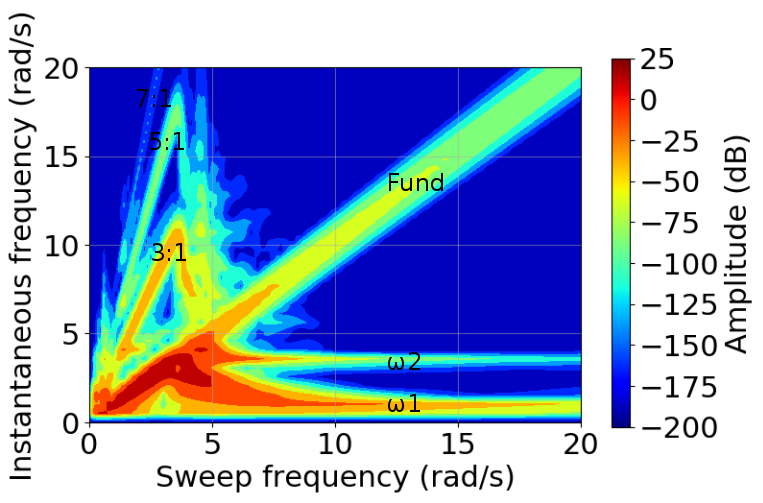
\includegraphics[width=\linewidth]{wt/2dof_wtnlin.png}
    \caption{}
  \end{subfigure}
  ~
  \begin{subfigure}[b]{0.48\textwidth}
    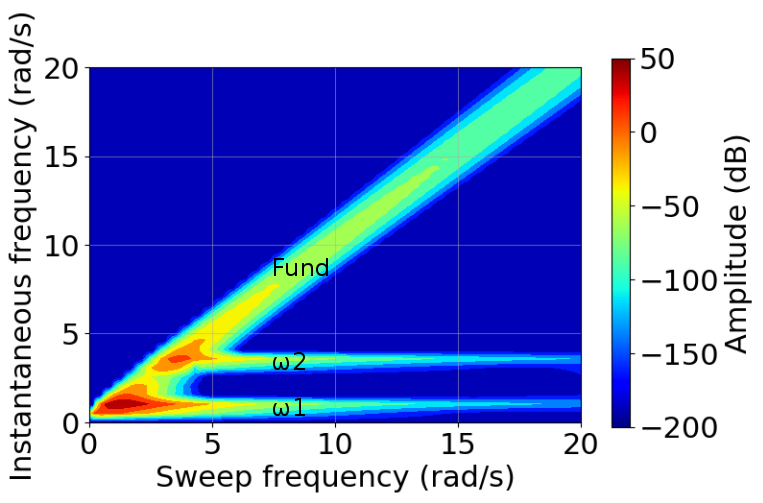
\includegraphics[width=\linewidth]{wt/2dof_wtlin.png}
    \caption{}
  \end{subfigure}
  \\
  \begin{subfigure}[b]{0.49\textwidth}
    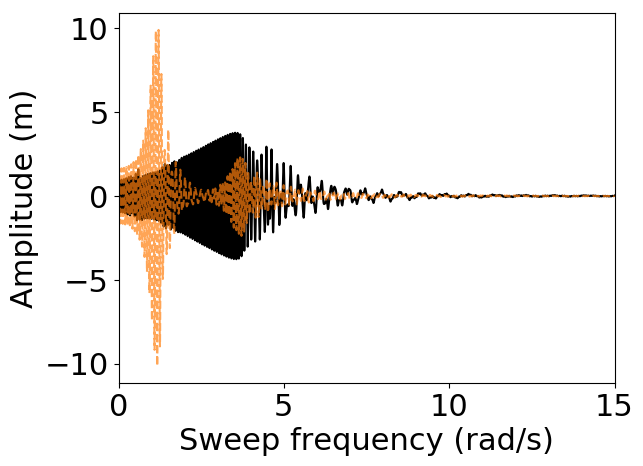
\includegraphics[width=\linewidth]{wt/2dof_wtsweep.png}
    \caption{}
  \end{subfigure}
  \begin{subfigure}[b]{0.49\textwidth}
    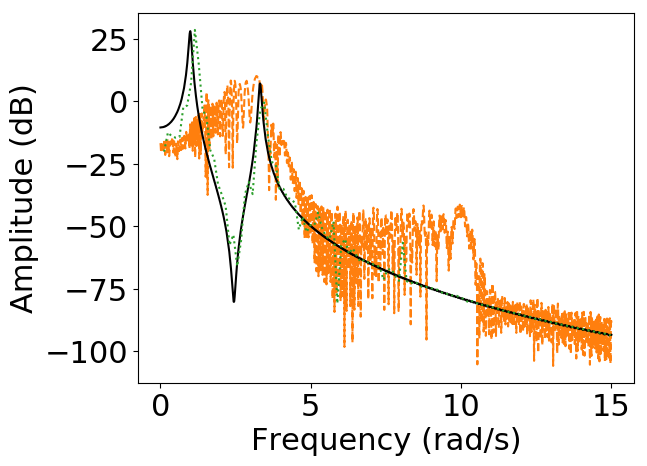
\includegraphics[width=\linewidth, height=5.5cm]{wt/2dof_wtfrf.tikz}
    \caption{}
  \end{subfigure}
  \caption{Morlet wavelet transform of a sine sweep of the coupled duffing
    system. Shown for $x_1$.
    \textbf{(a)}: MW of the nonlinear system;
    \textbf{(b)}: MM of the underlaying linear system;
    \textbf{(c)}: Sine sweep of
    \sampleline{}(nonlinear) and
    \textcolor{orange}{\sampleline{dashed}(linear)} system;
    \textbf{(d)}: Fourier transform of the
    \sampleline{}(nonlinear) and
    \textcolor{orange}{\sampleline{dashed}(linear)} system.
    \textcolor{green}{\sampleline{dotted}(nonlinear multisine)} is the FRF of a
    multisine excitation of the nonlinear system.
  }
  \label{fig:mw_2dof}
\end{figure}


\subsection{Summary}
\label{sec:wt_transform}

The WM shows the instantaneous frequency content of a time signal. Varying
frequency content is a sign of nonlinear vibration and the way the spectra
changes might give clues to the type of nonlinearity.
The frequency spectra is changed in the following way by nonlinear components:

\begin{itemize}
\item \textit{Dissipative NLs} does not affect the resonance frequencies much.
\item \textit{Hardening (softening) elastic NLs} increase (softens) the resonance
  frequencies with amplitude.
\item \textit{Assymmetric elastic NLs} generate even harmonic components.
\item \textit{Symmetric elastic NLs} generate uneven harmonic components.
\item \textit{Nonsmooth elastic NLs} generates wideband frequency components.
\end{itemize}

%%% Local Variables:
%%% mode: latex
%%% TeX-master: "../../report"
%%% End:
